\section{Вращательное движение твердого тела}

\begin{wrapfigure}{r}{2.5cm}
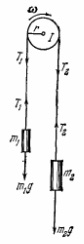
\includegraphics{0701RotationDynamicsAtwoodMachine.jpg}
\end{wrapfigure}

%1
\AddProb Определить ускорение тел и натяжение нити на машине Атвуда, предполагая, что $m_2>m_1$. 
Момент инерции блока относительно геометрический оси равен $I$, радиус блока $r$. Массу нити считать пренебрежимо малой. 

\AddProb Монета массы $m$ и радиуса $r$, вращаясь в горизонтальной плоскости вокруг своей геометрической оси с угловой скоростью $\omega$, 
вертикально падает на горизонтальный диск и прилипает к нему. В результате диск приходит во вращение вокруг своей оси. 
Возникающий при этом момент сил трения в оси диска постоянен и равен $M_0$. Через какое время вращение диска прекратится? 
Сколько оборотов сделает диск до полной остановки? Момент инерции диска относительно его геометрической оси~$I_0$. 
Расстояние между осями диска и монеты равно~$d$.

\AddProb Сплошной однородный короткий цилиндр радиуса $r$, вращающийся вокруг своей геометрической оси со скоростью $n$ об/с, 
ставят в вертикальном положении на горизонтальную поверхность. Сколько оборотов $N$ сделает цилиндр, прежде чем вращение его полностью прекратится? 
Коэффициент трения скольжения между основанием цилиндра и поверхностью, на которую он поставлен, не зависит от скорости вращения и равен~$\mu$.

\begin{wrapfigure}{r}{2cm}
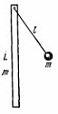
\includegraphics{0704RotationDynamicsBarAndBall.jpg}
\end{wrapfigure}

\AddProb Тонкий стержень массы $m$ и длины $L$ подвешен за один конец и может вращаться без трения вокруг горизонтальной оси. 
К той же оси подвешен на нити дины $l$ шарик такой же массы $m$. Шарик отклоняют на некоторый угол и отпускают. 
При какой длине нити шарик после удара о стержень остановится? Удар абсолютно упругий.

\AddProb Однородный тонкий негнущийся стержень массой $m$ поддерживается в горизонтальном положении двумя вертикальными опорами у концов стержня. 
В начальный момент времени $t$~ =~0 одна из опор выбивается. Найти силу, которая действует на вторую опору сразу же после этого момента.

\begin{figure}[h]
\centering
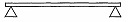
\includegraphics{0705RotationDynamicsHorisontalBar.jpg}
\end{figure}

\begin{wrapfigure}{r}{2.5cm}
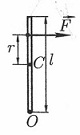
\includegraphics{0706RotationDynamicsSword.jpg}
\end{wrapfigure}

%6
\AddProb Каким участком сабли следует рубить лозу, чтобы рука не чувствовала удар? Саблю считать однородной пластиной.

\AddProb Шарик массой $m$ летит со скоростью $u_0$ навстречу покоящемуся стержню массой $M = 2m$ и длиной $2L$. 
Направление движения шарика перпендикулярно стержню и удалено на расстояние $l$ от его центра. 
После удара скорость шарика становится равной $u_1$, а стержня -- $V$. При этом стержень начинает вращаться с угловой скоростью $\omega$. 
Требуется определить 1) при каком $l$ шарик после удара остановится, а также 
2) скорость шарика, стержня и угловую скорость вращения стержня, если шарик ударяет в конец стержня.

\AddProb (2003 год) Обруч радиуса $R$ бросают вперед со скоростью $v_0$ и сообщают ему одновременно угловую скорость $\omega_0$. 
Определить минимальное значение угловой скорости, при котором обруч после движения с проскальзыванием покатится назад. 
Найти значение конечной скорости $v$, если $\omega_0 > \omega_{0min} $. Трением качения можно пренебречь.

\begin{wrapfigure}{r}{4cm}
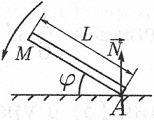
\includegraphics{0709RotationDynamicsFallOfBar.jpg}
\end{wrapfigure}

\AddProb Тонкий стержень массой $M$ и длиной $L$ свободно падает в вертикальной плоскости из начального положения, 
в котором угол между стержнем и горизонтальной плоскостью составлял $30^{\circ}$. 
Определите давление стержня на плоскость в момент удара, считая точку опоры стержня о плоскость неподвижной.

\AddProb Сплошной цилиндр без проскальзывания катится со скоростью $v$ по горизонтальной плоскости, 
которая переходит в наклонную поверхность с углом $\alpha$. Радиус цилиндра $R$. Какова должна быть $v$, чтобы цилиндр "не прыгнул"?

%11
\AddProb (2004) Двум дискам радиусами $R_1$ и $R_2$ сообщили одну и ту же угловую скорость $\omega_0$,
 а затем их привели в соприкосновение, и система через некоторое время пришла в новое установившееся состояние движения. 
Оси дисков неподвижны, трения в осях нет. Моменты инерции относительно их осей вращения равны $I_1$ и $I_2$. 
Найти приращение момента импульса системы и приращение ее механической энергии.

\AddProb Как надо ударить кием по бильярдному шару, чтобы при столкновении с другим (неподвижным) шаром 
1) оба шара стали двигаться вперед (удар с накатом), 2) первый шар остановился, а второй двигался вперед (удар с остановкой), 
3) второй шар двигался вперед, а первый откатился назад (удар с оттяжкой)? 
Предполагается, что удар наносится горизонтально в вертикальной плоскости, проходящей через центр шара и точку касания его с плоскостью бильярдного стола.

%Рассмотрим движение двух бильярдных шаров. Первым шаром назовем тот, по которому игрок ударяет кием, а вторым -- тот, 
%в который игрок старается попасть первым шаром. Как надо ударить кием, чтобы при столкновении первого шара со вторым: 
%1) оба шара стали двигаться вперед (удар с накатом), 2) первый шар остановился, а второй стал двигаться вперед (удар с остановкой), 
%3) второй шар двигался вперед, а первый откатился назад (удар с оттяжкой)? 
%Предполагается, что удар наносится горизонтально в вертикальной плоскости, проходящей через центр шара и точку касания его с плоскостью бильярдного стола.

\AddProb (2007) На гладком горизонтальном столе лежит однородный твердый стержень длины $l$ и массы $M$, 
в край которого ударяет твердый шарик массы $m$, движущийся со скоростью $v_0$, перпендикулярной к оси стержня. 
Считая удар идеально упругим и предполагая, что силы трения между поверхностью стола и лежащими на ней телами пренебрежимо малы, 
вычислить угловую скорость вращения стержня после удара.

\AddProb (2008) Сплошной однородный цилиндр, ось которого горизонтальна, движется без вращения по гладкой горизонтальной плоскости в направлении, 
перпендикулярном к его оси. В некоторый момент цилиндр достигает границы, где поверхность становится шероховатой и возникает постоянная 
(не зависящая от скорости) сила трения скольжения, а трение качения отсутствует. Каково будет движение цилиндра после перехода границы? 
Как распределится кинетическая энергия поступательного движения цилиндра?

\AddProb (2001) Пуля массы $m$, летящая горизонтально, попадает в покоящийся на шероховатой горизонтальной поверхности деревянный шар массой 
$M >> m$  и радиусом $R$ на расстоянии $l $ ниже центра масс и застревает в нем. Найти установившуюся скорость шара.

%16
\AddProb (2002) Шарик массой $m$ подвешен на нерастяжимой нити длиной $l$ и отклонен на малый угол от положения равновесия. 
В той же точке, что и нить, подвешен стержень длиной $1.5l$. Какова должна быть масса стержня $M$, чтобы в результате столкновения шарик остановился? 
Удар абсолютно упругий. Определить период колебаний шарика.

\begin{wrapfigure}{r}{4cm}
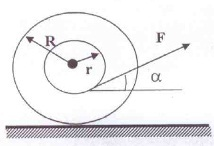
\includegraphics[width=4cm]{0717RotationDynamicsReelOfThread.jpg}
\end{wrapfigure}

\AddProb (2010) На горизонтальной шероховатой поверхности лежит катушка ниток массой $m$. 
Ее момент инерции относительно собственной оси $I$, внешний радиус $R$, радиус намотанного слоя ниток $r$. 
Катушку без скольжения начали тянуть с постоянной силой $F$, направленной под углом $\alpha$ к горизонту. Найти ускорение центра катушки.